%label:"art:lagrangiancobordisms"
%author:JeffHicks
%name:"lagrangian cobordisms"
%type:"article"

If $M$ is a manifold, a \emph{surgery of $M$} is the replacement of a $D^{n-k}\times S^k$ with $S^{n-k-1}\times D^{k+1}$. 
Surgery of manifolds is closely tied to cobordisms between manifolds. 
Let $M, N$ be $n$-manifolds. 
A \emph{cobordism} $K: M\rightsquigarrow N$ is a manifold with boundary $\partial K=M\sqcup N$. 
There is an analogous notion of cobordism exists for Lagrangian submanifolds.
%tag:000K
%label:def:lagrangianCobordism
%author:JeffHicks
%name:"differential graded module"
%type:definition
%source:arnol1980lagrange



Let $\{L_0, \ldots, L_k\}$ be Lagrangian submanifolds of $X$. 
A \emph{Lagrangian cobordism} with ends $L_0, \ldots L_k$ is a Lagrangian submanifold $K\subset X\times T^*\RR$ for which there exists a compact subset $D\subset \CC$ so that : 
        \[K\setminus( \pi_\CC^{-1}(D))=\bigcup_{i=0}^k L_i\times \ell_i.\]
    Here, the $\ell_i$ are rays of the form $\ell_i(t)=i\cdot \jmath +t$, where $t\in \RR_{\geq 0}$.
We denote such a cobordism $K:(L_1, \ldots L_k)\rightsquigarrow L_0$. 
\label{def:lagrangianCobordism}


One can also discuss Lagrangian cobordisms with both positive and negative ends.
%tag:000X
%label:"fig:lagrangianCobordism"
%author:JeffHicks
%name:"Lagragian cobordism"
%type:"figure"
%parent:def:lagrangianCobordism
%caption:"The projection of a Lagrangian cobordism $K\subset X\times \CC$ to the $\CC$ factor. This cobordism has ends  $K:(L_0, L_1, \ldots L_k)\rightsquigarrow \emptyset."




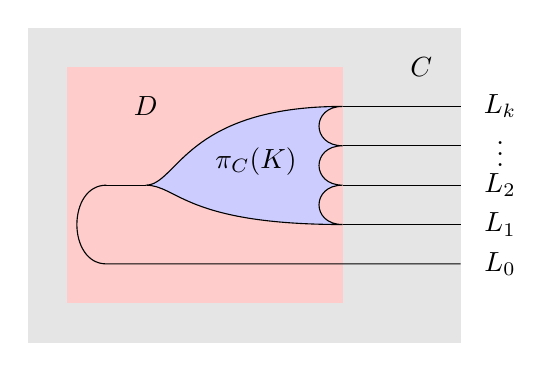
\begin{tikzpicture}[xscale=-1]
    \fill[fill=gray!20]  (-2,-2.5) rectangle (3.5,1.5);
    \fill[red!20]  (-0.5,-2) rectangle (3,1);
        \draw[fill=blue!20] (-0.5,-1) .. controls (-0.1,-1) and (-0.1,-0.5) .. (-0.5,-0.5) .. controls (-0.1,-0.5) and (-0.1,0) .. (-0.5,0) .. controls (-0.1,0) and (-0.1,0.5) .. (-0.5,0.5) .. controls (1.5,0.5) and (1.6,-0.5) .. (2,-0.5) .. controls (1.6,-0.5) and (1.5,-1) .. (-0.5,-1);
        \draw (-2,-1) -- (-0.5,-1);
        \draw (-2,-0.5) -- (-0.5,-0.5);
        \draw (-2,0) -- (-0.5,0);
        \draw (-2,0.5) -- (-0.5,0.5);
        \draw (2,-0.5) -- (2.5,-0.5);
        \node at (-2.5,0.5) {$L_k$};
        \node at (-2.5,0) {$\vdots$};
        \node at (-2.5,-0.5) {$L_2$};
        \node at (-2.5,-1) {$L_1$};
        \node at (-2.5,-1.5) {$L_0$};
        \node at (0.6,-0.2) {$\pi_{\mathbb C}(K)$};
    \draw (2.5,-0.5) .. controls (3,-0.5) and (3,-1.5) .. (2.5,-1.5) .. controls (2,-1.5) and (-1.5,-1.5) .. (-2,-1.5);
    
    \node at (2,0.5) {$D$};
    \node at (-1.5,1) {$\mathbb C$};
    \end{tikzpicture}
%label:"exm:suspensionCobordism"
%author:JeffHicks
%name:"suspension of exact homotopy"
%type:"example"
%source:"audin1994symplectic"

    Let $\li_s: L\times \RR_t\to X$ be an exact Lagrangian homotopy generated by the function $H_t: L\times \RR_t\to \RR$. 
    The \emph{suspension} of $H_t$ is the Lagrangian cobordism $K_{H_t}$ with topology $L\times \RR$ parameterized by 
    \begin{align*}
          L\times \RR\to & X\times \CC\\
           (u, s)\mapsto& (\li_t(u), s+\jmath H_t(u))\in X\times \CC.
    \end{align*}

%tag:000K
%label:exm:polterovichSurgeryTrace
%author:JeffHicks
%name:"Polterovich surgery trace"
%type:example



    Let $L_1, L_2\subset X$ be Lagrangian submanifolds which intersect transversely at a point $q$, so we can define the Polterovich surgery $L_1\#_q L_2$. 
    Then there exists a Lagrangian cobordism $(L_1\#_U L_2)\rightsquigarrow (L_1, L_2)$. 
    \label{prop:traceconstruction}

Lagrangian cobordisms give us new examples of exact sequences in the Fukaya category. 
%label:"thm:exactSequencesFromCobordisms"
%author:JeffHicks
%name:"Lagrangian cobordisms give exact sequences"
%type:"theorem"
%source:"biran2014lagrangian"

See also \cite{tanaka2016fukaya}.
Let $L_0, \ldots L_k\in \Fuk(X)$ be Lagrangian submanifolds, and suppose there exists a monotone Lagrangian cobordism $K: (L_0, \ldots, L_k)\rightsquigarrow \emptyset$. Then there exists an iterated cone decomposition in $\text{mod}-\Fuk(X)$,
%label:"dig:exactSequencesFromCobordisms"
%type:"diagram"
%author:JeffHicks
%name:"exact sequences from cobordisms"

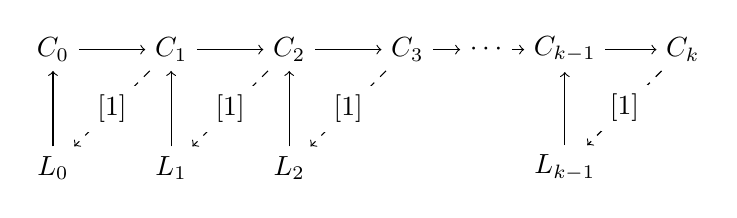
\begin{tikzpicture}




    \node (v1) at (1.5,-0.5) {$C_0$};
    \node (v2) at (3,-0.5) {$C_1$};
    \node (v3) at (4.5,-0.5) {$C_2$};
    \node (v4) at (6,-0.5) {$C_3$};
    \node (v6) at (8,-0.5) {$C_{k-1}$};
    \node (v7) at (9.5,-0.5) {$C_k$};
    \node (v8) at (1.5,-2) {$L_0$};
    \node (v9) at (3,-2) {$L_1$};
    \node (v10) at (4.5,-2) {$L_2$};
    \node (v11) at (8,-2) {$L_{k-1}$};
    \node (v5) at (7,-0.5) {$\cdots$};
    \draw[->]  (v1) edge (v2);
    \draw[->]  (v2) edge (v3);
    \draw[->]  (v3) edge (v4);
    \draw[->]  (v4) edge (v5);
    \draw[->]  (v5) edge (v6);
    \draw[->]  (v6) edge (v7);
    \draw[->]  (v8) edge (v1);
    \draw[->]  (v9) edge (v2);
    \draw[->]  (v10) edge (v3);
    \draw[->]  (v11) edge (v6);
    \draw[->,dashed]  (v2) edge  node[fill=white]{$[1]$} (v8);
    \draw[->,dashed]  (v3) edge  node[fill=white]{$[1]$} (v9);
    \draw[->,dashed]  (v4) edge  node[fill=white]{$[1]$} (v10);
    \draw[->,dashed]  (v7) edge  node[fill=white]{$[1]$}  (v11);
    \end{tikzpicture}
where each triangle in the diagram an exact triangle, $C_0=0$, and $C_k=k$.

In particular, if $K: (L_0, L_1, L_2)\rightsquigarrow \emptyset$ is a Lagrangian cobordism, then we have an exact triangle
\[L_2\to L_1\to L_0.\]
In contrast to \cref{cor:surgeryExactTriangle}, such a Lagrangian cobordism does not identify \emph{which} exact triangle one has --- it only identifies that you have an exact triangle. 
The iterated mapping cone given in \cref{thm:exactSequencesFromCobordisms} is an example of a twisted complex.